\documentclass{beamer}
\usetheme{PaloAlto}

\usepackage[utf8]{inputenc}
\usepackage{graphicx}

\title[c4]{A broken C compiler with a LLVM backend}
\author{Philipp Möller, Sam Courts, Yulia Iforgothername}
\date{March 2013}

\begin{document}
\frame{\titlepage}

\begin{frame}
  \frametitle{Table of Contents}
  \tableofcontents
\end{frame}

\section{Software Quality}

\begin{frame}
  \frametitle{Developing C++ Software}
  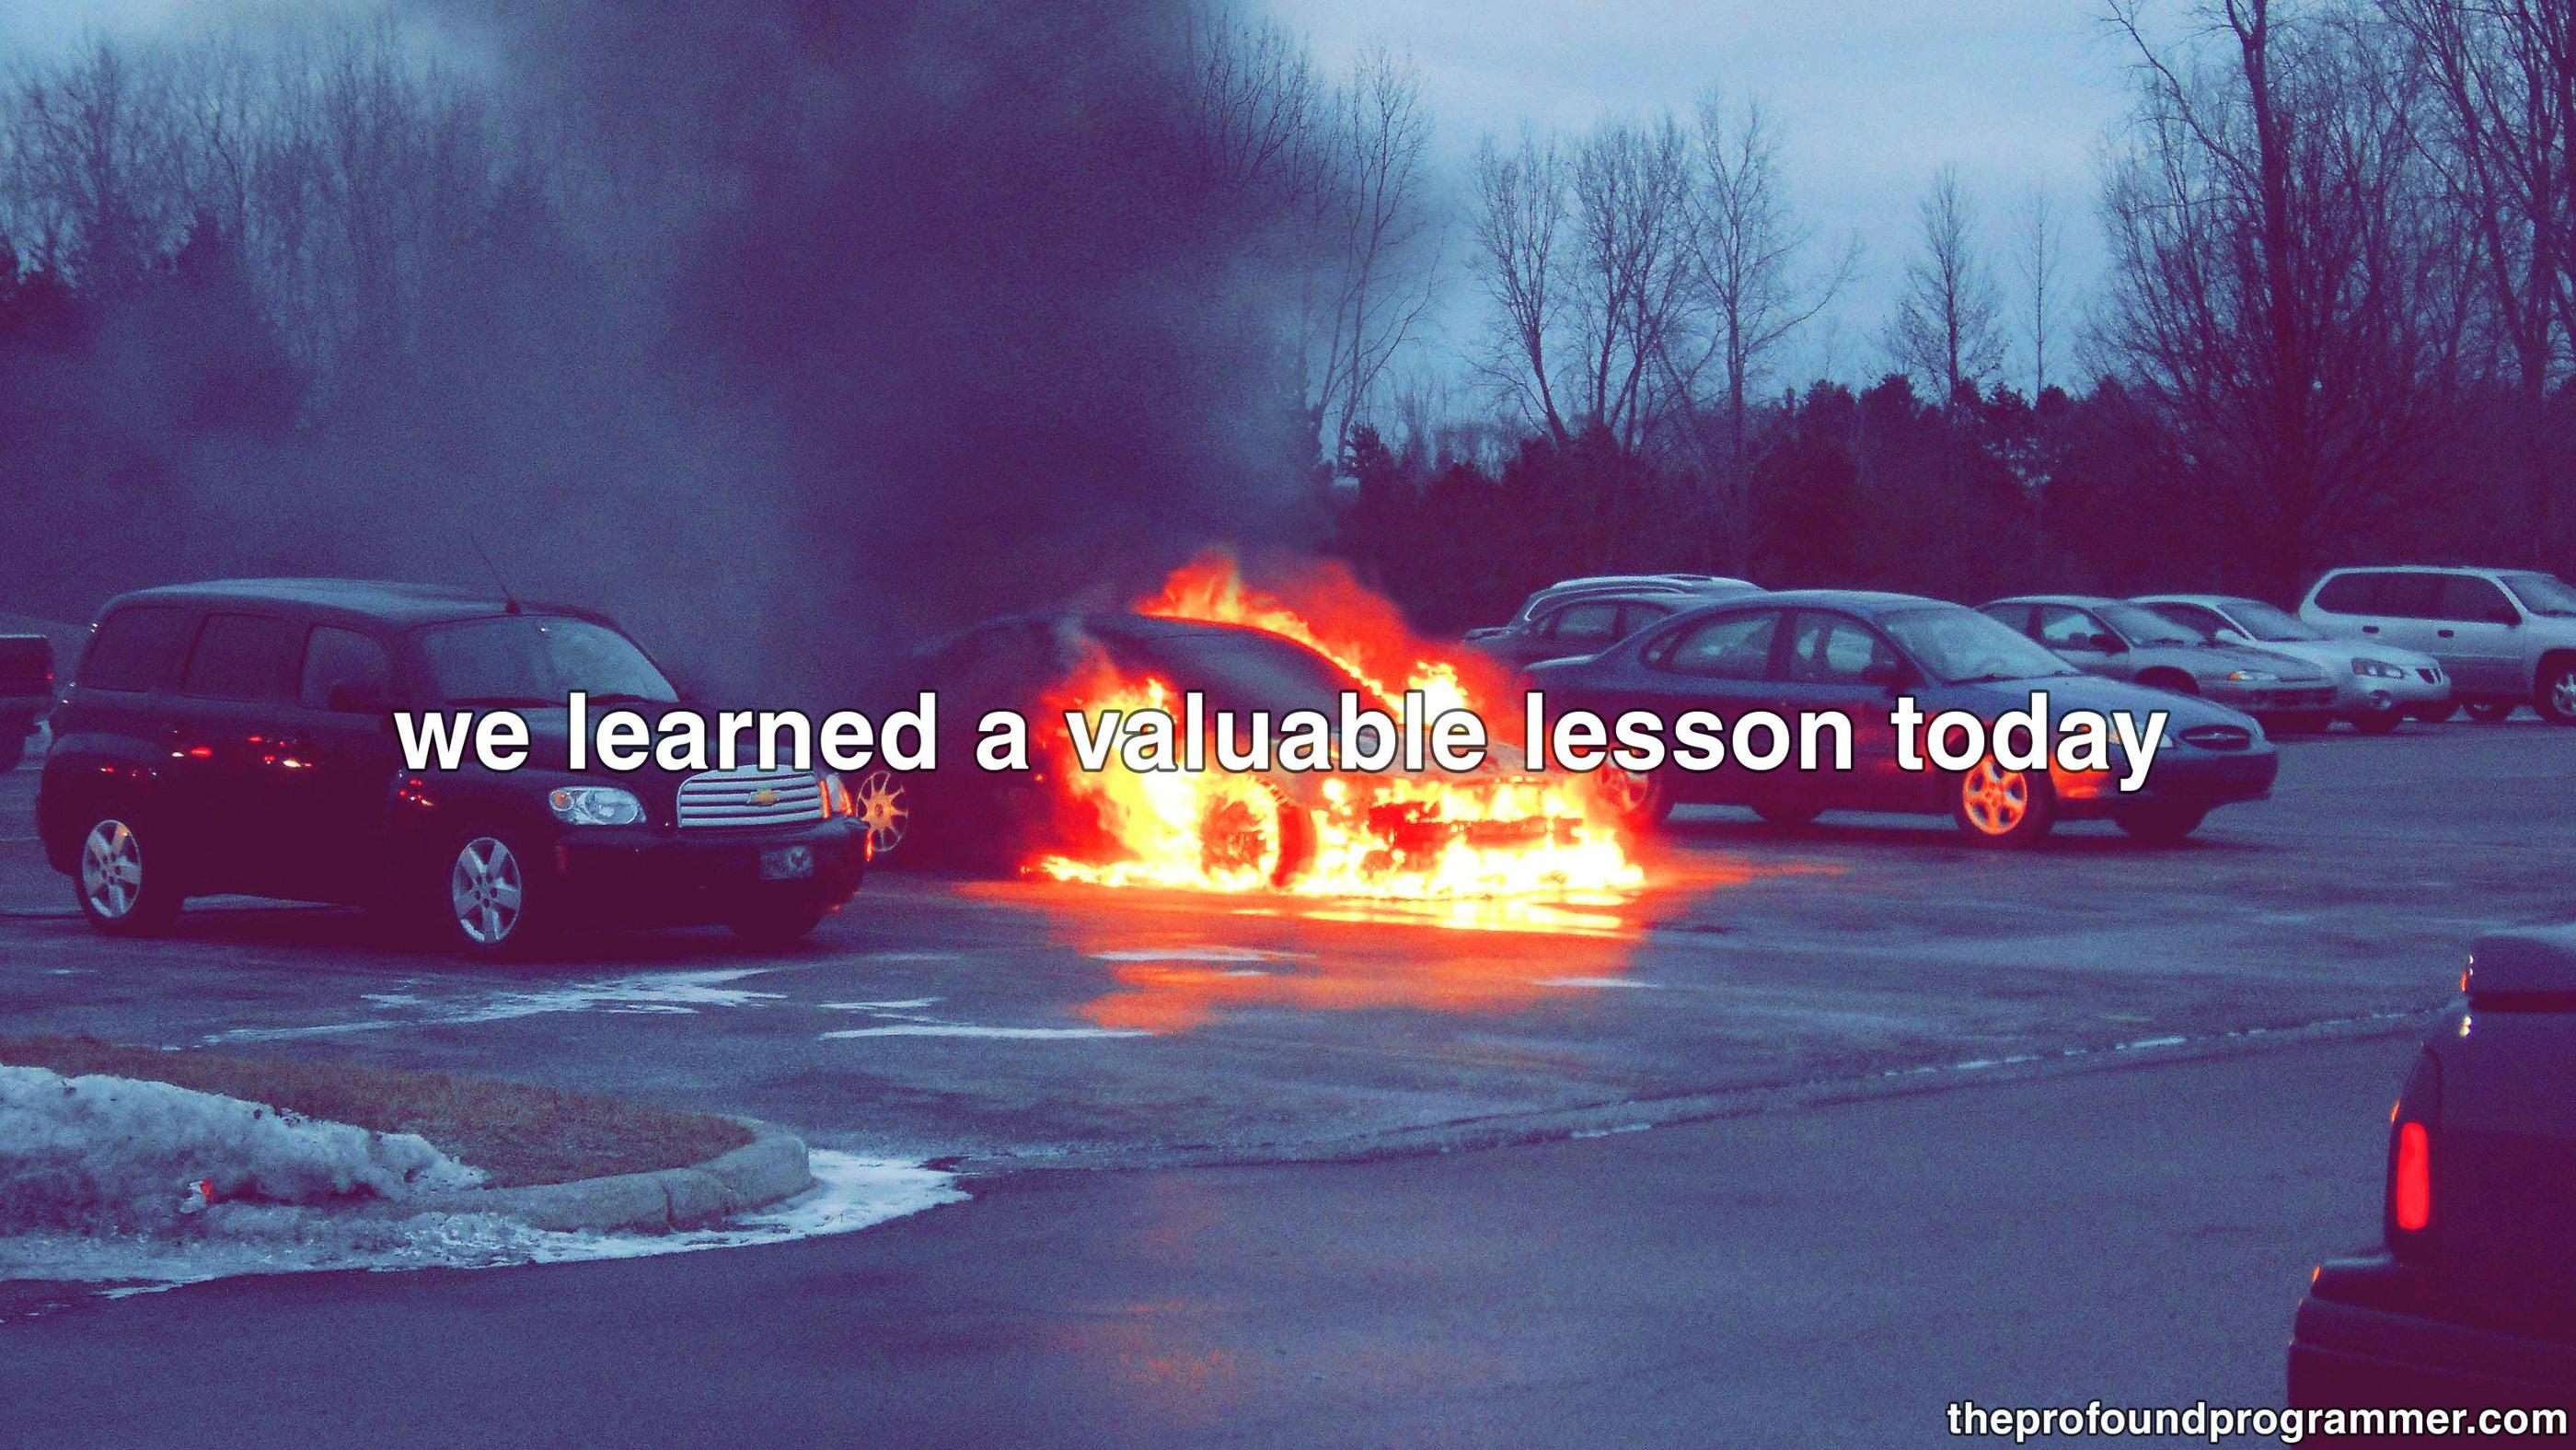
\includegraphics[scale=0.1]{valuable_lesson}
\end{frame}

\begin{frame}
  \frametitle{Tool Up}
  \begin{itemize}
  \item \tt{clang} + \tt{fsanitize}
  \item \tt{valgrind}
  \item \tt{gprof}
  \item use depending on programmer mood
  \end{itemize}
\end{frame}

\begin{frame}
  \frametitle{Automated Testing}
  \begin{itemize}
  \item $ \mathit{Make} + \mathit{diff} \equiv \mathit{test\_runner} $
  \item separate tests by compiler stages
  \item no real test plan $\rightarrow$ test as we go
  \item project was missing a tester
  \item $\sim{}100$ tests
  \end{itemize}
\end{frame}

\begin{frame}
  \frametitle{Coding Standards}
  \begin{itemize}
  \item<2-> just kidding...
  \item<3-> make sure no one is too far behind on C++ knowledge + implementation
  \end{itemize}
\end{frame}

\section{Lexer}

\begin{frame}
  \frametitle{Lexer}
  \begin{itemize}
  \item pretty simple
  \item \tt{mmap}'d inputs
  \item \tt{llvm::StringRef} to minimize copies
  \item good performance (even though it uses \tt{iostreams})
  \end{itemize}
\end{frame}

\section{Parser}
\begin{frame}
  \frametitle{The AST}
  \begin{itemize}
  \item boring pile of polymorphism in absence of a proper safe, stack-based discriminated union
  \item implementing \tt{boost::variant} fun, but daunting
  \item \tt{binary\_operator} not sub-classed
  \item \tt{base\_decl} to factor common decls, 
  \item no \tt{\{named|function|variable\}\_decl} $rightarrow$ not smart
  \end{itemize}
\end{frame}

\begin{frame}
  \frametitle{Parsing}
  \begin{itemize}
  \item allocates small nodes like crazy
  \item broken down into subparsers
  \item $1$ look-ahead, uber fast lexer $\rightarrow$ no caching
  \item split into multiple parsers sub-classed \tt{parser\_base}
  \end{itemize}
\end{frame}

\begin{frame}
  \frametitle{Printing}
  \begin{itemize}
  \item use visitor to easily introspect polymorphic hierarchies and
    delegate traversal
  \item told not to use visitors $\rightarrow$ good reason to use them
  \item already too much working code written $\rightarrow$ don't touch it
  \end{itemize}
\end{frame}

\section{Sema}
\begin{frame}
  \frametitle{Type Hierarchy}
  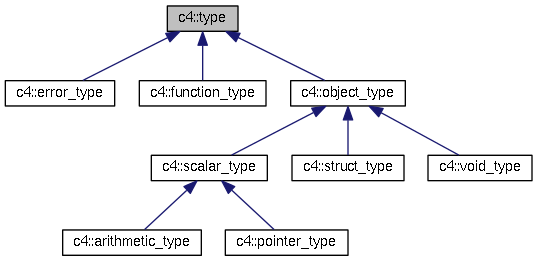
\includegraphics[scale=0.5]{type_hier}
\end{frame}

\begin{frame}
  \frametitle{Types}
  \begin{itemize}
  \item sema visitor attaches types to AST nodes
  \item use type singletons, where possible
  \end{itemize}
\end{frame}


\begin{frame}
  \frametitle{Scope}
  \begin{itemize}
  \item separate \{tag|variable\} scopes
  \item never duplicate struct type $\rightarrow$ easy to deal with completeness and equality
  \end{itemize}
\end{frame}

\section{Backend}
\begin{frame}
\end{frame}

\section{Optimizer}
\begin{frame}
\end{frame}

\end{document}

